\chapter{Υλικά και Μέθοδοι}

Σε αυτή την ενότητα θα περιγράψουμε την διαδικασία με την οποία συλλέχθηκαν τα δεδομένα αλλά και την πορεία της επεξεργασίας τους ώστε να εξαχθούν τα επιθυμητά αποτελέσματα. Όπως φαίνεται στην εικόνα \ref{fig:methods-process1} αρχικά συλλέγονται τα δεδομένα με την βοήθεια της συσκευής \eng{Kinect}, αλλά και των εξωτερικών δυνάμεων αν είναι υπαρκτές. Τα δεδομένα αυτά προτού επεξεργαστούν στα μετέπειτα στάδια φιλτράρονται κατάλληλα ώστε να μειωθούν οι ανεπιθύμητες παρεμβολές του θορύβου. Έπειτα ακολουθεί η διαδικασία της αντίστροφης κινηματικές, που με την βοήθεια ενός μοντέλου εξάγονται οι γενικευμένες συντεταγμένες (γωνίες) στις αρθρώσεις. Με χρήση αριθμητικών μεθόδων παραγογίζουμε δύο φορές το αποτέλεσμα ώστε να έχουμε στην διάθεση μας τις γενικευμένες ταχύτητες και επιταχύνσεις των αρθρώσεων του μοντέλου. Εφαρμόζουμε αντίστροφη δυναμική και εξάγουμε τις γενικευμένες ροπές στις αρθρώσεις που απαιτούνται για να παράξουν την δοσμένη κίνηση. Τέλος, έχοντας προσδώσει τους κατάλληλους μύες στο μοντέλο με βάση την γεωμετρία, αλλά και της δυναμικής τους, μπορούν να εκτιμηθούν οι δυνάμεις που ασκεί ο κάθε μυς.

\begin{figure}[H]
    \centering
    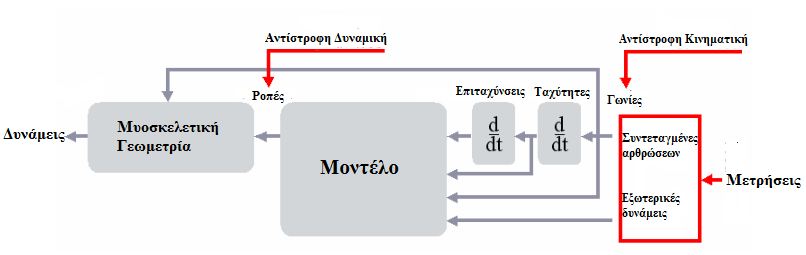
\includegraphics[width=1.0\textwidth]{methods/fig/process.png}
    \caption{Διαδικασία εξαγωγής των δυνάμενων}
    \label{fig:methods-process1}
\end{figure}

%%%%%%%%%%%%%%%%%%%%%%%%%%%%%%%%%%%%%%%%%%%%%%%%%%%%%%%%%%%%%%%%%%%%%%%%%%%%%%%%
\section{Καταγραφή της Κίνησης}

Όπως αναφέραμε χρησιμοποιούμε το \eng{Kinect} για την συλλογή των τροχιών των αρθρώσεων για μια δοσμένη κίνηση. Για την ανίχνευση του σκελετού εκμεταλλευόμαστε τον αλγόριθμο που είναι υλοποιημένος εσωτερικά στην συσκευή και έχουμε στην διάθεση μας στις τρισδιάστατες συντεταγμένες των αρθρώσεων. Το λογισμικό που χρησιμοποιείται για την καταγραφή της κίνησης έχει υλοποιηθεί στην \eng{C++} και βασίζεται στην βιβλιοθήκη της \eng{Microsoft} για το \eng{Kinect} (\eng{Microsoft Kinect SDK}). Επιπλέον, γίνεται χρήση φίλτρων για την εξομάλυνση του θορύβου και του τρέμουλο (\eng{jitter}). Τα αποτελέσματα μπορούν να καταγραφούν σε διαφορετικούς τύπους αρχείων, ώστε να χρησιμοποιηθούν στα μετέπειτα στάδια της ανάλυσης.

%%%%%%%%%%%%%%%%%%%%%%%%%%%%%%%%%%%%%%%%%%%%%%%%%%%%%%%%%%%%%%%%%%%%%%%%%%%%%%%%
\section{Δημιουργία του Μοντέλου}

Πριν περιγράψουμε την διαδικασία της δημιουργίας του μοντέλου θα ήθελα να αναφερθώ στα εργαλεία που χρησιμοποιήθηκαν. Για την μοντελοποίηση αλλά και την διεξαγωγή των αναλύσεων χρησιμοποιήθηκε το ανοιχτό εργαλείο-βιβλιοθήκη \eng{OpenSim}. Το \eng{OpenSim} είναι μια πλατφόρμα που βασίζεται στην μηχανή \eng{SimTK Simbody} για την μοντελοποίηση, προσομοίωση και ανάλυση νευρομυοσκελετικών συστημάτων \cite{delp07}. Το εργαλείο διαθέτει γραφική διεπαφή, αλλά και διεπαφή για τον προγραμματιστή σε γλώσσα \eng{C++}. Είναι δυνατή η επέκταση του λογισμικού με την βοήθεια \eng{plugins}. Το \eng{OpenSim} χρησιμοποιείται ευρέως από την επιστημονική κοινότητα κυρίως σε βιοϊατρικές εφαρμογές. Η κοινότητα διαθέτει μεγάλο αριθμό από έτοιμα μοντέλα, πειραματικά δεδομένα και επιπρόσθετα εργαλεία για την διεξαγωγή των αναλύσεων.

\begin{figure}[H]
    \centering
    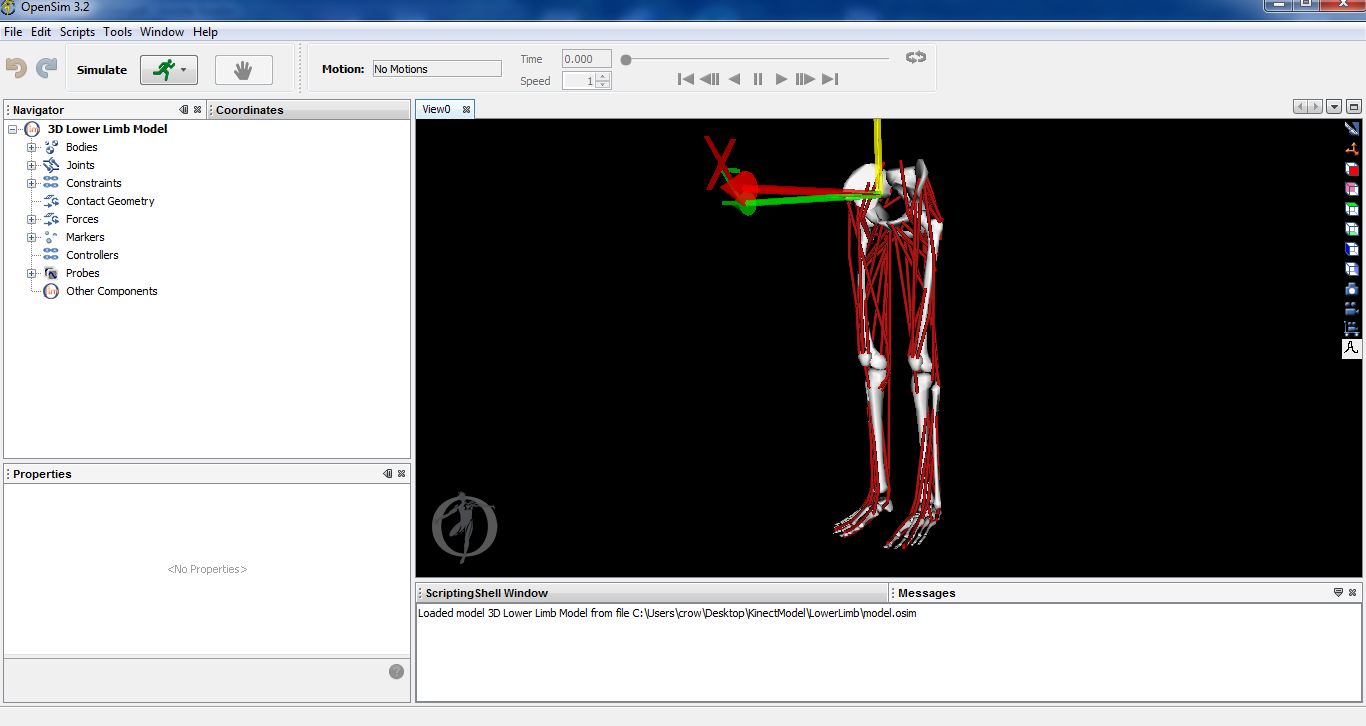
\includegraphics[width=0.8\textwidth]{methods/fig/opensim.png}
    \caption{Γραφική διεπαφή του \eng{OpenSim}}
    \label{fig:opensim-gui}
\end{figure}

Δεν θα μπορούσα να παραλείψω βέβαια και το \eng{Simbody}, το οποίο είναι η καρδιά της πλατφόρμας. Σαν μηχανή φυσικής, δίνει την δυνατότητα περιγραφής πολύπλοκων διατάξεων με έναν μεγάλο αριθμό από έτοιμα στοιχεία όπως είναι η μοντελοποίηση δυνάμενων, εισαγωγή περιορισμών στην κίνηση, περιγραφή της διάταξης, ποικίλα τύπων βαθμών ελευθερίας και άλλα πολλά. Έχει σχεδιαστεί κατάλληλα ώστε να ωθεί την αποδοτικότητα και παράλληλα να μην μειώνει την ευελιξία. Είναι ένα εργαλείο που σου δίνει την δυνατότητα να περιγράφεις και να προσομοιώσεις τα φαινόμενα που μελετάς.

Όσον αφορά τις δυνατότητες που προσφέρει η προγραμματιστική βιβλιοθήκη του \eng{OpenSim} μπορούμε να διακρίνουμε κάποια βασικά χαρακτηριστικά \ref{fig:opensim-architecture}. Βλέπουμε ότι στην βάση βρίσκεται το \eng{Simbody}. Επιπλέον, έχει δοθεί η δυνατότητα περιγραφής του μοντέλου και επιπρόσθετα στοιχεία που βοηθούν στο να γίνει η ανάλυση. Το \eng{OpenSim} βοηθάει στο να γίνει η περιγραφής της σκελετικής διάταξης, να προδοθούν βαθμοί ελευθερίας και περιορισμοί στην κίνηση. Ακόμη υπάρχει η δυνατότητα μοντελοποίησης των μυών και η προσθήκη τους στην διάταξη. Όπως θα δούμε και στην συνέχει μπορούν να εξαχθούν πληθώρα είδη αναλύσεων, που μπορούν να χρησιμοποιηθούν ακόμη και σε ιατρικές εφαρμογές, αλλά και όχι μόνο.

\begin{figure}[H]
    \centering
    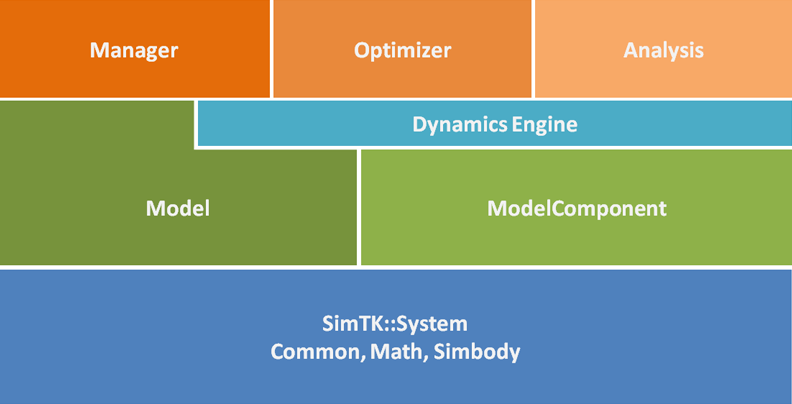
\includegraphics[width=0.8\textwidth]{methods/fig/opensim-architecture.png}
    \caption{Συνοπτική αρχιτεκτονική της βιβλιοθήκης του \eng{OpenSim}}
    \label{fig:opensim-architecture}
\end{figure}

%%%%%%%%%%%%%%%%%%%%%%%%%%%%%%%%%%%%%%%%%%%%%%%%%%%%%%%%%%%%%%%%%%%%%%%%%%%%%%%%
\subsection{Επεξήγηση του Μοντέλου}

Για την διεξαγωγή των προσομοιώσεων είναι αναγκαία η σχεδίαση ενός μοντέλου που θα είναι όσο το δυνατών πιο αντιπροσωπευτικό σε σχέση με το πραγματικό. Η διαδικασία είναι πολύπλοκη και απαιτεί γνώσεις όχι της μόνο φυσιολογίας του ανθρώπου, αλλά και γνώσεις ώστε να περιγραφεί η λειτουργία του μοντέλου. Στην παρούσα μελέτη έχει μοντελοποιηθεί το τμήμα των κάτω άκρα του ανθρώπου, ώστε να γίνει η μελέτη κατά την διεξαγωγή κινήσεων.

Το μοντέλο αποτελείται από 20 βαθμούς ελευθερίας, από τους οποίους οι 6 έχουν να κάνουν με τον προσανατολισμού και την περιστροφή της λεκάνης, που είναι και η ρίζα της ιεραρχίας. Οπότε έχουμε άλλους 7 βαθμούς ελευθερίας για κάθε πόδι. Επίσης το μοντέλο διαθέτει 43 μύες για κάθε πόδι οι οποίοι είναι τοποθετημένοι με βάση την πραγματική τους γεωμετρία γύρω από τα οστά. Οι μύες είναι σε θέσει να παράξουν έργο στις καθαρισμένες αρθρώσεις ώστε να παραχθεί η επιθυμητή κίνηση. Επίσης, λόγο της έλλειψης δεδομένων που αφορούν τις εξωτερικές δυνάμεις αντίδρασης από το δάπεδο κατά την κίνηση έχει γίνει η κατάλληλη μοντελοποίηση τους με χρήση δυνάμεων επαφής. Το μοντέλο έχει δημιουργηθεί στα πλαίσια μελέτης πως μπορεί μια εγχείρηση να αλλάξει τις παραμέτρους των μυών και κατά συνέπεια το αποτέλεσμα της βάδισης με βάση το \cite{delp90} και τροποποιήθηκε κατάλληλα στην παρούσα εργασία.

\begin{figure}[H]
    \centering
    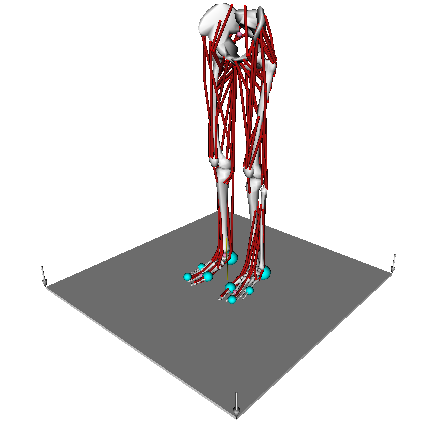
\includegraphics[height=0.38\textheight]{methods/fig/lower-limb-model.png}
    \caption{Μυοσκελετικό μοντέλο μαζί και δάπεδο αντίδρασης}
    \label{fig:lower-limb-model}
\end{figure}

\begin{center}
    \begin{tabular}{ccc}
        \toprule
        % after \\: \hline or \cline{col1-col2} \cline{col3-col4} ...
        Άρθρωση & Κάτω όριο & Πάνω όριο\\
        \midrule
        \eng{pelvis\_till (z)} & $-90^{o}$ & $+90^{o}$\\
        \eng{pelvis\_list (x)} & $-90^{o}$ & $+90^{o}$\\
        \eng{pelvis\_rotation (y)} & $-90^{o}$ & $+90^{o}$\\
        \eng{pelvis\_tx} & $-5$ & $+5$\\
        \eng{pelvis\_ty} & $-1$ & $+2$\\
        \eng{pelvis\_tz} & $-3$ & $+3$\\
        \eng{hip\_flexion} & $-95^{o}$ & $+95^{o}$\\
        \eng{hip\_adduction} & $-50^{o}$ & $+15^{o}$\\
        \eng{hip\_rotation} & $-20^{o}$ & $+20^{o}$\\
        \eng{knee\_angle} & $-120^{o}$ & $+0^{o}$\\
        \eng{ankle\_angle} & $-30^{o}$ & $+30^{o}$\\
        \eng{subtalar\_angle} & $-20^{o}$ & $+20^{o}$\\
        \eng{mtp\_angle} & $-30^{o}$ & $+30^{o}$\\
        \bottomrule
    \end{tabular}
    \captionof{table}{Βαθμοί ελευθερίας με τους αντίστοιχους περιορισμούς}
    \label{tab:model-dof}
\end{center}

Όπως φαίνεται και στον πίνακα \ref{tab:model-dof} παρουσιάζονται οι βαθμοί ελευθερίας του μοντέλου μαζί με τους περιορισμούς στην επιτρεπτή κίνηση. Ο γοφός έχει τρις περιστροφικούς βαθμούς, το γόνατο έναν, ο αστράγαλος δύο και τα δάχτυλα των ποδιών έναν. Η λεκάνη φροντίζει να προσανατολίσει και να τοποθετήσει κατάλληλα το μοντέλο στο χώρο και στην πραγματικότητα δεν παίζει κάποιο ρόλο στην κίνηση. Αυτός ο πλεονασμός της λεκάνη είναι μια από της τροποποιήσεις του αρχικού μοντέλου ώστε να μπορεί να βρεθεί το κάτω τμήμα σε διαφορετικές διατάξεις στον χώρο.

Η έλλειψη εξωτερικών δυνάμεων αντίδρασης από το δάπεδο είναι σοβαρό μειονέκτημα που οδηγεί σε προσεγγίσεις της πραγματικότητας. Αναγκαστικά υιοθετήθηκαν τεχνικές εκτίμησης των δυνάμεων με μοντελοποίηση της επαφής με το δάπεδο \cite{seitha11}. Το \eng{OpenSim} χρησιμοποιεί δύο τύπων δυνάμεων επαφής που έχουν υλοποιηθεί από το \eng{Simbody}. Η πρώτη είναι η \eng{Hunt Crossley Force} που βασίζεται στην θεωρία επαφής του \eng{Hertz} \cite{hunt75}. Αυτή η μέθοδος υπολογίζει την ελαστική παραμόρφωση αναλυτικά και το \eng{Simbody} υποστηρίζει κάποια βασικά γεωμετρικά σχήματα. Στην μοντελοποίηση που κάναμε έχει χρησιμοποιηθεί μια επιφάνεια για το δάπεδο και έχουν τοποθετηθεί σφαίρες στις πατούσες. Η εναλλακτική λύση είναι η αναπαράσταση της γεωμετρίας με πλέγματα (\eng{mesh}) τα οποία αποτελούνται από ελατήρια για την μοντελοποίηση της ελαστικότητας \cite{hertz82}.

\begin{figure}[H]
    \centering
    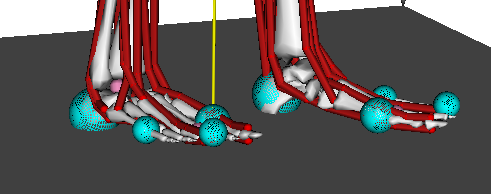
\includegraphics[width=0.8\textwidth]{methods/fig/foot-contact.png}
    \caption{Εποπτική αναπαράσταση των σφαιρών αντίδρασης στα πόδια}
    \label{fig:foot-contact}
\end{figure}

Όσον αφορά τους μύες, έχουν τροποποιηθεί ώστε να χρησιμοποιούν το έτοιμο μοντέλο μυ \eng{Millard2013EquilibriumMuscle} που είναι υλοποιημένο στην βιβλιοθήκη του \eng{OpenSim}. Οι παράμετροι των μυών (μέγιστη παραγόμενη δύναμη, βέλτιστο μήκος μυ, μήκος χαλαρότητας του τένοντα, σχετική γωνία μεταξύ μυ και τένοντα, γεωμετρία) έχουν προσδιοριστεί από το αρχικό μοντέλο και είναι συμβατά με το νέο μοντέλο μυ.

%%%%%%%%%%%%%%%%%%%%%%%%%%%%%%%%%%%%%%%%%%%%%%%%%%%%%%%%%%%%%%%%%%%%%%%%%%%%%%%%
\section{Προετοιμασία για την Αντίστροφη Κινηματική}

Αφού έχει καταγραφεί μια κίνηση και υπάρχει το αντίστοιχο μοντέλο μπορεί να λυθεί το πρόβλημα της αντίστροφης κινηματικής ώστε να προσδιορισθούν οι γενικευμένες συντεταγμένες (συνήθως γωνίες) για την δοσμένη κίνηση. Προτού όμως εκτελέσουμε την αντίστροφη κινηματική πρέπει να γίνουν κάποια επιπλέον βήματα.

%%%%%%%%%%%%%%%%%%%%%%%%%%%%%%%%%%%%%%%%%%%%%%%%%%%%%%%%%%%%%%%%%%%%%%%%%%%%%%%%
\subsection{Τοποθέτηση Ενδείξεων}

Αρχικά πρέπει να προσδιοριστούν αντιστοιχίες μεταξύ της καταγεγραμμένης κίνησης και του μοντέλου. Ωστόσο μην ξεχνάμε ότι το πρόβλημα της αντίστροφης κινηματικής προσπαθεί να βρει τις γωνίες που πρέπει να τροφοδοτήσει το μοντέλο ώστε να ταιριάξει με την δοσμένη διάταξη της κίνησης. Αφού τα πειράματα έγινα με την βοήθεια του \eng{Kinect}, έχουμε στην διάθεση μας τις θέσεις των αρθρώσεων. Συνεπώς, πρέπει να τοποθετηθούν οι αντίστοιχες ενδείξεις και στο μοντέλο.

\begin{figure}[H]
    \centering
    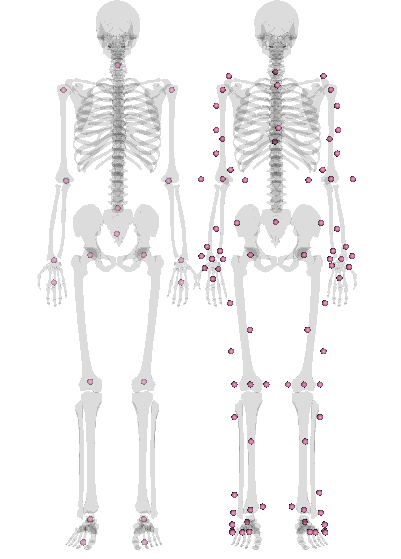
\includegraphics[height=0.6\textheight]{methods/fig/kinect-vicon-markers.png}
    \caption{Σύγκριση συστήματος ενδείξεων του \eng{Kinect} και του \eng{Vicon} δεξιά}
    \label{fig:kinect-vicon-markers}
\end{figure}

Στην εικόνα \ref{fig:kinect-vicon-markers} με ροζ χρώμα συμβολίζεται οι ενδείξεις (\eng{marker}). Από αριστερά βλέπουμε τις ενδείξεις που απαιτούνται για να συνδεθεί η καταγεγραμμένη κίνηση από το \eng{Kinect}, ενώ από δεξιά βλέπουμε τους δείκτες που απαιτούνται για να γίνει μια καταγραφή από ένα επαγγελματικό σύστημα της εταιρίας \eng{Vicon}. Οι ενδείξεις προσδιορίζονται με βάση την εφαρμογή, ωστόσο λόγο ότι ο προσανατολισμός και η θέση στο χώρο ενός τμήματος του σώματος, όπως είναι τα οστά, απαιτεί ώστε να βρεθεί μοναδική λύση τουλάχιστον τρία μη συνευθειακά σημεία σε κάθε τμήμα. Αυτός είναι και ο λόγος για τον οποίον ο δεξής σκελετός έχει πιο πολλές ενδείξεις. Αυτό είναι και ένα βασικό μειονέκτημα του συστήματος μας σε σχέση με επαγγελματικά συστήματα, δηλαδή για κάποιες κινήσεις μπορεί να μην βρεθεί ο σωστός προσανατολισμός. Ωστόσο για απλές κινήσεις το αποτέλεσμα της αντίστροφης κινηματικής δίνει ικανοποιητικά αποτελέσματα για την διάταξη μας, αν συγκρίνουμε και το αντίστοιχο κόστος το να έχει κανείς ένα επαγγελματικό σύστημα.

%%%%%%%%%%%%%%%%%%%%%%%%%%%%%%%%%%%%%%%%%%%%%%%%%%%%%%%%%%%%%%%%%%%%%%%%%%%%%%%%
\subsection{Κανονικοποίησης του Μοντέλου}

Το τελευταίο πράγμα που πρέπει να γίνει είναι η κανονικοποίησης του γενικού μοντέλου που έχουμε στην διάθεση μας, ώστε να αρμόζει σε διαφορετικά σωματότυπα. Το \eng{OpenSim} διαθέτει δυνατότητα μετατροπής του μοντέλου αλλά και την θέση των ενδείξεων από το γενικό στο ειδικό μοντέλο. Η διαδικασία είναι σχετικά απλή και βελτιώνει σημαντικά το αθροιστικό σφάλμα της αντίστροφης κινηματικής. Με βάση τις ενδείξεις που έχουν τοποθετηθεί στο γενικό μοντέλο γίνεται μια δημιουργία ζευγαριών που αντιπροσωπευθούν κάποιο τμήμα του σώματος (π.χ. η ένδειξη του γοφού και του γονάτου αντιστοιχεί στο μηριαίο οστό) και θα ληφθούν υπόψη ώστε να γίνει ομαλή μεταβολή του τμήματος, για να ταιριάξει στις μετρήσεις.

Έχει γίνει κατάλληλη επιλογή των τμημάτων και των ζευγαριών ενδείξεων ώστε να μεταβληθούν κατάλληλα όλα τα τμήματα του σώματος. Επίσης δίνεται η δυνατότητα να διατηρηθεί η μάζα του γενικού μοντέλου. Το γενικό μοντέλο αντιπροσωπευθεί άντρα ύψους 1.80\eng{cm} και ζυγίζει 75\eng{kg}. Το κάτω τμήμα που έχει παρθεί ζυγίζει 41\eng{kg}. Η μάζα και η αδράνεια κάθε οστού έχει προσδιοριστεί για το γενικό μοντέλο και τροποποιείται ανάλογα με βάση τις μετρήσεις.

\begin{center}
    \begin{tabular}{ccc}
        \toprule
        Τμήμα του σώματος & 1η ένδειξη & 2η ένδειξη\\
        \midrule
        \eng{pelvis} & \eng{HIP\_RIGHT} & \eng{HIP\_LEFT}\\
        \eng{femru} & \eng{HIP} & \eng{KNEE}\\
        \eng{tibia} & \eng{KNEE} & \eng{ANKLE}\\
        \eng{calcn} & \eng{ANKLE} & \eng{FOOT}\\
        \bottomrule
    \end{tabular}
    \captionof{table}{Τμήματα του σώματος και τα ζευγάρια των ενδείξεων για τα κάτω άκρα}
    \label{tab:scale-pairs}
\end{center}

%%%%%%%%%%%%%%%%%%%%%%%%%%%%%%%%%%%%%%%%%%%%%%%%%%%%%%%%%%%%%%%%%%%%%%%%%%%%%%%%
\subsection{Διεξαγωγή της Αντίστροφης Κινηματικής}

Αφού έχουν γίνει τα παραπάνω πλέων μπορεί να εκτελεστεί η αντίστροφη κινηματική και να παραχθούν οι γωνίες που απαιτούνται για την παραγωγή της δοσμένης κίνησης από το μοντέλο. Το αποτέλεσμα την αντίστροφης κινηματικής είναι ζωτικής σημασίας για τα μετέπειτα στάδια της ανάλυσης. Οι υπολογισμένες γωνίες αν αναπαρασταθούν δεν θα πρέπει να έχουν απότομες μεταβολές από μια στιγμή σε άλλη, ώστε να μην παράγουν μη φυσιολογικές επιταχύνσεις και με αποτέλεσμα δυνάμεις. Κατά την εύρεση λύσεων υπάρχουν γωνίες για τις οποίες η διάταξη βρίσκεται σε απροσδιοριστία μορφή. Το τελευταίο μπορεί να αποφευχθεί αν εισαχθούν οι κατάλληλοι περιορισμοί στις κινήσεις της διάταξης αφότου έχει μελετηθεί εκ των προτέρων. 

Κατά την διεξαγωγή της αντίστροφης κινηματικής μαζί με το κανονικοποιημένο μοντέλο τροφοδοτούμε και τις συντεταγμένες που έχουμε καταγράψει από το \eng{Kinect}, οι οποίες βρίσκονται σε κατάλληλη μορφή (*.\eng{trc}) που υποστηρίζεται από το \eng{OpenSim}. 

%%%%%%%%%%%%%%%%%%%%%%%%%%%%%%%%%%%%%%%%%%%%%%%%%%%%%%%%%%%%%%%%%%%%%%%%%%%%%%%%
\section{Προσδιορισμός των Γενικευμένων Ροπών}

Αφού έχουμε στην διάθεση μας τα αποτελέσματα της αντίστροφης κινηματικής το επόμενο βήμα είναι ο προσδιορισμός των γενικευμένων ροπών στις αρθρώσεις του μοντέλου. Ας υπενθυμίσουμε την σχέση που περιγράψαμε \ref{equ:dynamics-equation}, που αποτελεί την λύση του προβλήματος. Τα απαραίτητα στοιχεί είναι οι εξωτερικές δυνάμεις.